\chapter{Modelo matemático}

\section{Modelo cinemático}
\subsection{Matriz de transformación homogénea}



\begin{figure}
    \centering
    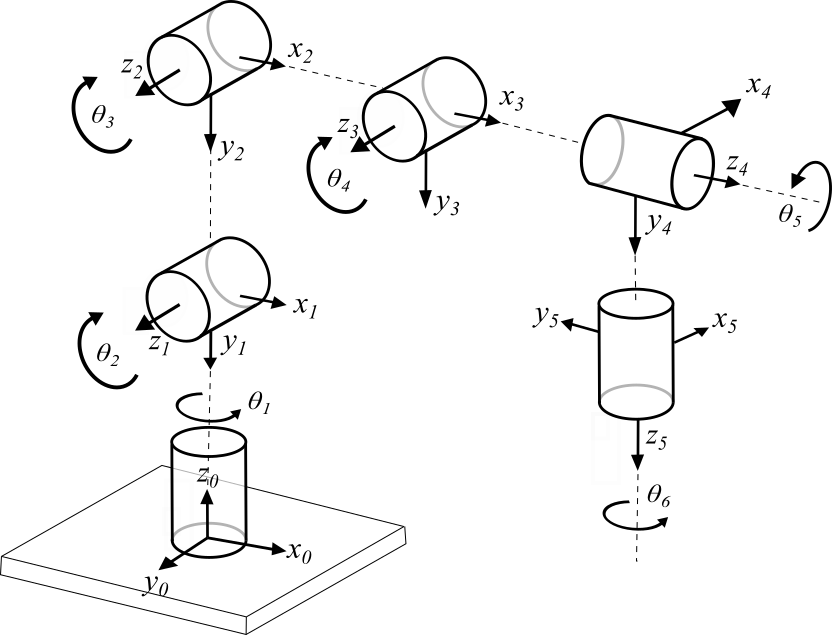
\includegraphics[width=\textwidth]{./img/chapter4/kinematicchainv5.png}
    \caption{Cadena cinemática ¿free body diagram?}
    \label{fig:kinematicchain}
\end{figure}



\[
{}_{0}^{1}T = 
\begin{bmatrix}
    1 & 0 & 0 & {a}_x  \\
    0 & \cos{\theta_1} & -\sin{\theta_1} & {a}_y \\
    0 & \sin{\theta_1} & \cos{\theta_1} & {a}_z \\
    0 & 0 & 0 & 1
\end{bmatrix}
\]

% Como no hay rotación en el frame, se usa la matriz identidad.

\[
{}_{1}^{2}T = 
\begin{bmatrix}
    1 & 0 & 0 & b_x  \\
    0 & 1 & 0 & b_y \\
    0 & 0 & 1 & b_z \\
    0 & 0 & 0 & 1
\end{bmatrix}
\]

% Como no hay rotación en el frame, se usa la matriz identidad.

\[
{}_{2}^{3}T = 
\begin{bmatrix}
    1 & 0 & 0 & c_x  \\
    0 & 1 & 0 & c_y \\
    0 & 0 & 1 & c_z \\
    0 & 0 & 0 & 1
\end{bmatrix}
\]

\[
{}_{3}^{4}T = 
\begin{bmatrix}
    \cos{\theta_4} & 0 & \sin{\theta_4} & d_x  \\
    0 & 1 & 0 & d_y \\
    -\sin{\theta_4} & 0 & \cos{\theta_4} & d_z \\
    0 & 0 & 0 & 1
\end{bmatrix}
\]

\[
{}_{4}^{5}T = 
\begin{bmatrix}
    1 & 0 & 0 & e_x  \\
    0 & \cos{\theta_5} & -\sin{\theta_5} & e_y \\
    0 & \sin{\theta_5} & \cos{\theta_5} & e_z \\
    0 & 0 & 0 & 1
\end{bmatrix}
\]

\[
{}_{0}^{5}T = {}_{0}^{1}T {}_{1}^{2}T {}_{2}^{3}T {}_{3}^{4}T {}_{4}^{5}T 
\]

\subsection{Convención de Denavit Hartenberg}


\begin{table}[h]
\centering
\caption{Parámetros Denavit Hartenberg}
 \label{table:denavithartenberg}
\begin{tabular}{l|l|l|l|l|}
               & $\theta$ [rad] & a [m]    & d [m]   & $\alpha$ [rad]                        \\ 
\hline
Articulación 1 & 0                           & 0        & 0.1519  & $\frac{\pi}{2}$   \\
Articulación 2 & 0                           & -0.24365 & 0       & 0                                                  \\
Articulación 3 & 0                           & -0.21325 & 0       & 0                                                  \\
Articulación 4 & 0                           & 0        & 0.11235 & $\frac{\pi}{2}$   \\
Articulación 5 & 0                           & 0        & 0.08535 & $-\frac{\pi}{2}$  \\
Articulación 6 & 0                           & 0        & 0.0819  & 0                                                 
\end{tabular}
\end{table}